\documentclass[12pt]{article}
\usepackage{fontspec}
\usepackage{fullpage}
\usepackage{hyperref}
\usepackage{array}
\usepackage{url}
\usepackage{amsmath}
\usepackage{pgfplotstable}
\usepackage{algorithm2e}
\usepackage{multirow}
\usepackage{subcaption}
\usepackage{color}
\usepackage{adjustbox}
\usepackage{tikz}
\usepackage{tikz-dependency}
\usetikzlibrary{shapes,fit,calc,er,positioning,intersections,decorations.shapes,mindmap,trees}
\tikzset{decorate sep/.style 2 args={decorate,decoration={shape backgrounds,shape=circle,
      shape size=#1,shape sep=#2}}}

\newfontfamily\hebfont[Script=Hebrew, Scale=MatchUppercase]{FreeSans}
\newcommand{\heb}[1]{\bgroup\textdir TRT\hebfont #1\egroup}

\title{Universal Semantic Parsing with Neural Networks \\
\heb{ניתוח סמנטי אוניברסלי באמצעות רשתות נוירונים}
}
\date{2018 \heb{דצמבר}}

\begin{document}

\maketitle

\begin{table}[!th]\small
\begin{tabular}{lr>{\bfseries}r}
Daniel Hershcovich & \heb{דניאל הרשקוביץ} & \heb{שם התלמיד:} \\
Prof. Ari Rappoport and Dr. Omri Abend & \heb{פרופ' ארי רפופורט וד"ר עמרי אבנד} & \heb{שמות המדריכים:}
\end{tabular}
\end{table}



\section{Introduction}\label{sec:introduction}

Semantic applications in natural language processing (e.g., machine translation)
require understanding the meaning of text.
Syntactic representations suffer from limitations, since they do not
represent semantic structure directly,
which semantic annotation schemes attempt to do.
In order to represent the full range of semantic structures exhibited by
natural language, three properties should be supported: reentrancy,
representing arguments shared between predicates (Figure~\ref{fig:graduation});
non-terminal nodes for multi-word units (Figure~\ref{fig:home});
and discontinuity of semantic units in the text (Figure~\ref{fig:gave}).
The only semantic annotation scheme that supports the combination of these criteria is UCCA
\cite{abend2013universal}.

\begin{figure}[ht]\small
  \begin{subfigure}{.6\textwidth}
  \parbox{.1\textwidth}{\caption{}\label{fig:graduation}}
  \parbox{.3\textwidth}{
  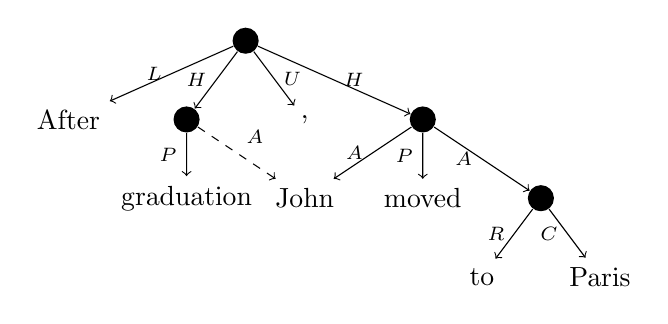
\begin{tikzpicture}[level distance=10mm, ->]
    \node (ROOT) [fill=black, circle] {}
      child {node (After) {After} edge from parent node[left] {\scriptsize $L$}}
      child {node (graduation) [fill=black, circle] {}
      {
        child {node {graduation} edge from parent node[left] {\scriptsize $P$}}
      } edge from parent node[left] {\scriptsize $H$} }
      child {node {,} edge from parent node[right] {\scriptsize $U$}}
      child {node (moved) [fill=black, circle] {}
      {
        child {node (John) {John} edge from parent node[left] {\scriptsize $A$}}
        child {node {moved} edge from parent node[left] {\scriptsize $P$}}
        child {node [fill=black, circle] {}
        {
          child {node {to} edge from parent node[left] {\scriptsize $R$}}
          child {node {Paris} edge from parent node[left] {\scriptsize $C$}}
        } edge from parent node[left] {\scriptsize $A$} }
      } edge from parent node[right] {\scriptsize $H$} }
      ;
    \draw[dashed,->] (graduation) to node [auto] {\scriptsize $A$} (John);
  \end{tikzpicture}
  }
  \end{subfigure}
  \begin{subfigure}{.4\textwidth}
  \parbox{.1\textwidth}{\caption{}\label{fig:home}}
  \parbox{.3\textwidth}{
  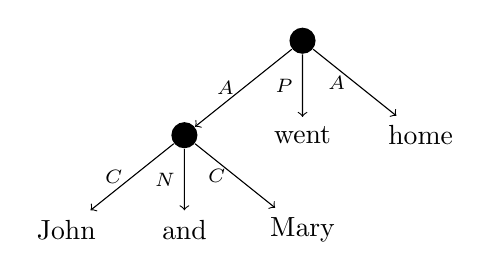
\begin{tikzpicture}[level distance=12mm, ->,
      every node/.append style={midway}]
    \node (ROOT) [fill=black, circle] {}
      child {node [fill=black, circle] {}
      {
        child {node {John} edge from parent node[left] {\scriptsize $C$}}
        child {node {and} edge from parent node[left] {\scriptsize $N$}}
        child {node {Mary} edge from parent node[left] {\scriptsize $C$}}
      } edge from parent node[left] {\scriptsize $A$} }
      child {node {went} edge from parent node[left] {\scriptsize $P$}}
      child {node {home} edge from parent node[left] {\scriptsize $A$}}
      ;
  \end{tikzpicture}
  }
  \end{subfigure}
  \begin{subfigure}{.4\textwidth}
  \parbox{.1\textwidth}{\caption{}\label{fig:gave}}
  \parbox{.3\textwidth}{
  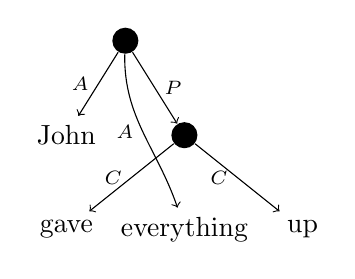
\begin{tikzpicture}[level distance=12mm, ->,
      every node/.append style={midway}]
    \node (ROOT) [fill=black, circle] {}
      child {node {John} edge from parent node[left] {\scriptsize $A$}}
      child {node [fill=black, circle] {}
      {
      	child {node {gave} edge from parent node[left] {\scriptsize $C$}}
      	child {node (everything) {everything} edge from parent[white]}
      	child {node {up} edge from parent node[left] {\scriptsize $C$}}
      } edge from parent node[right] {\scriptsize $P$} }
      ;
    \draw[bend right,->] (ROOT) to[out=-20, in=180] node [left] {\scriptsize $A$} (everything);
  \end{tikzpicture}
  }
  \end{subfigure}
  \begin{subfigure}{.6\textwidth}
  \parbox{.1\textwidth}{\caption{}\label{fig:shower}}
  \parbox{.3\textwidth}{
  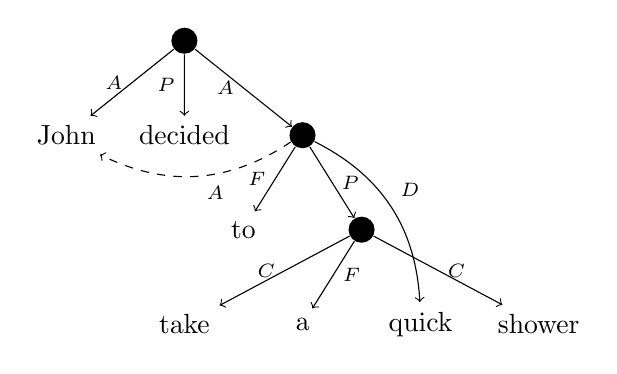
\begin{tikzpicture}[level distance=12mm, ->,
      every node/.append style={midway}]
    \node (ROOT) [fill=black, circle] {}
      child {node (John) {John} edge from parent node[left] {\scriptsize $A$}}
      child {node {decided} edge from parent node[left] {\scriptsize $P$}}
      child {node (totakeaquickshower) [fill=black, circle] {}
      {
        child {node {to} edge from parent node[left] {\scriptsize $F$}}
        child {node [fill=black, circle] {}
        {
          child {node {take} edge from parent node[left] {\scriptsize $C$}}
          child {node {a} edge from parent node[right] {\scriptsize $F$}}
          child {node (quick) {quick} edge from parent[white]}
          child {node {shower} edge from parent node[right] {\scriptsize $C$}}
        } edge from parent node[right] {\scriptsize $P$} }
      } edge from parent node[left] {\scriptsize $A$} }
      ;
    \draw[bend left,dashed,->] (totakeaquickshower) to node [auto] {\scriptsize $A$} (John);
    \draw[bend left,->] (totakeaquickshower) to node [auto] {\scriptsize $D$} (quick);
  \end{tikzpicture}
  }
  \end{subfigure}
  \caption{\label{fig:examples}
    UCCA examples.
    (\subref{fig:graduation}) includes a remote edge (dashed),
    resulting in ``John'' having two parents.
    (\subref{fig:home}) includes a coordination construction (``John and Mary'').
    (\subref{fig:gave}) includes a discontinuous unit (``gave ... up'').
    (\subref{fig:shower}) includes both a remote edge and a discontinuous unit (``take a ... shower'').
    Legend: $P$ -- Process (a Scene's main relation), $A$ -- Participant,
    $L$ -- inter-scene Linker, $H$ -- Parallel Scene, $C$ -- Center, $D$ -- Adverbial,
    $R$ -- Relator, $N$ -- Connector, $U$ -- Punctuation, $F$ -- Function unit.
  }
\end{figure}

Universal Cognitive Conceptual Annotation (UCCA)
is a cross-linguistically applicable semantic representation scheme.
It covers the predicate-argument
structures evoked by predicates of all grammatical categories, the inter-relations between them,
as well as other major linguistic phenomena.
UCCA has demonstrated applicability to multiple languages,
rapid annotation \cite{abend2017uccaapp},
stability in translation \cite{sulem2015conceptual}
and benefit for various applications
\cite{birch2016hume,choshen2018usim,sulem2018samsa,sulem2018simple}.

While semantic representation schemes are different in form and focus,
much of their semantic content is shared \cite{abend2017state}.
Recent work in semantic parsing has targeted
Abstract Meaning Representation \cite{banarescu2013abstract} and
Semantic Dependencies \cite{oepen2016towards}.
Universal Dependencies \cite{nivre2016universal}
is a \textit{syntactic} dependency scheme aiming for cross-lingual consistency,
whose annotation is often similar to the common practice in semantic treebanks
(Figure~\ref{fig:original_example_ud}).

\begin{figure}[th]
  \centering
    \begin{dependency}[text only label, label style={above,font=\tt}, font=\small]
    \begin{deptext}[column sep=.8em,ampersand replacement=\^]
    After \^ graduation \^ , \^ John \^ moved \^ to \^ Paris \\
    \end{deptext}
        \depedge[edge unit distance=1ex]{2}{1}{case}
        \depedge[edge unit distance=1ex]{4}{3}{punct}
        \depedge[edge unit distance=1ex]{5}{4}{nsubj}
        \depedge[edge unit distance=1ex, edge end x offset=-2pt]{2}{5}{obl}
        \depedge[edge unit distance=1ex]{7}{6}{case}
        \deproot[edge unit distance=1.5ex]{5}{root}
        \depedge[edge unit distance=1.5ex]{5}{7}{obl}
    \end{dependency}
\caption{Example UD tree, demonstrating practices common in semantic annotation:
linking content words to content words, and the preference of lexical heads over functional ones.
\label{fig:original_example_ud}}
\end{figure}

My research is concerned with learning to parse UCCA graphs from text, representing its semantics.
I introduce a general graph parser,
and investigate the relationship with other representations to find beneficial commonalities and
differences highlighting the potential utility of semantic parsers for text understanding applications.
The analysis also exposes challenges semantic parsers must address,
and potential sources for improvement.

\section{Goals}\label{sec:goals}

In my research, I pursue the following goals:

\begin{itemize}
  \item Developing techniques for general graph parsing.
    Specifically, devising a method for automatic prediction of UCCA
    structure given plain text.
  \item Investigating and quantifying the relationship between the content
    captured in UCCA and other semantic or syntactic representations.
  \item Taking advantage of the similarities to other schemes,
    to improve UCCA parsing by learning common distinctions.
\end{itemize}


\section{Methods}\label{sec:methods}

\subsection{Transition-Based Parsing}\label{sec:transition_based}

Transition-based parsers \cite{Nivre03anefficient} build trees or graphs
as they scan the text incrementally.
The parse is created by applying a \textit{transition} at each step to the parser state,
defined using three data structures: a buffer $B$ of tokens and nodes to be processed,
a stack $S$ of nodes currently being processed,
and a graph $G=(V,E,\ell)$ of constructed nodes and labeled edges.
Some of the states are marked as \textit{terminal}, meaning that $G$ is the final output.
A classifier is used at each step to select the next transition based on features
that encode the parser's current state.
During training, an oracle creates training instances for the classifier,
based on the gold-standard annotation.

The transition-based approach has produced some of the best
results in syntactic dependency parsing
\cite{kiperwasser2016simple,andor2016globally}, and has also demonstrated
strong performance in a variety of other semantic and syntactic settings
\cite{maier2015discontinuous,damonte-17}.
Transition-based methods are a natural starting point for UCCA parsing,
as the set of distinctions it represents, which is centered around predicate-argument
structures and their inter-relations, is similar in spirit to the distinctions
conveyed by dependency schemes.


\subsection{Neural Networks}\label{sec:neural_networks}

Over the past few years, neural networks have re-emerged as powerful
machine-learning models, yielding state-of-the-art results in fields such as image
recognition and speech processing. More recently, neural network models
started to be applied also to textual natural language signals, again with very
promising results \cite{goldberg2016primer}.
As the name suggest, they are
inspired by the brain's computation mechanism, which consists of computation
units called neurons.
Artificial neural networks operate on dense input representations
by linear and non-linear transformations, and combinations thereof.

When dealing with language data, it is very common to work with sequences, such
as words (sequences of letters), sentences (sequences of words) and documents.
Recurrent neural networks \cite{elman1990finding} allow representing
arbitrarily sized structured
inputs in a fixed-size vector, while paying attention to the structured
properties of the input.
Specifically, a bidirectional recurrent neural network (BiRNN) is
an extension of RNNs that take into account both the
past and the future. A specific flavor of RNN called a long short-term memory network
(LSTM) is very common as it yields strong results.


\section{Experiments}\label{sec:experiments}

\subsection{Experimental Setup}\label{sec:setup}

In my first experiment, I applied two methods for UCCA parsing:
one based on conversion to simpler structures and using existing parser,
and the other where I developed a novel transition-based BSS parser.

\paragraph{Data.}\label{sec:data}
The English UCCA-annotated corpora \cite{abend2013universal} is used
as a test case, in both in-domain and out-of-domain scenarios.
The in-domain data is taken from the UCCA Wikipedia corpus (henceforth, \textit{Wiki}),
and the out-of-domain data is taken from the English part of the UCCA
\textit{Twenty Thousand Leagues Under the Sea} English-French parallel corpus
(henceforth, \textit{20K Leagues}).\footnote{Both are available at
\url{http://www.cs.huji.ac.il/~oabend/ucca.html}}
Table~\ref{table:data} presents some statistics for the two corpora, demonstrating that while
the \textit{Wiki} corpus is over ten times larger, the overall statistics are
similar.
Passages of indices up to 655 of the \textit{Wiki} corpus are used as training
set, passages 656--700 as development set, and passages 701--695 as in-domain test set.
While UCCA edges can cross sentence boundaries, the common
practice in semantic parsing is to train parsers on individual sentences,
and so this was done here too.
Inter-relations between sentences are thus discarded (0.18\% of the edges).
Linkage nodes and edges are also discarded, as they often express
inter-sentence relations and are thus mostly redundant when applied at the
sentence level, as well as implicit nodes (see \S\ref{sec:introduction}).
In the out-of-domain experiments, the same parser
(trained on the \textit{Wiki} corpus) is applied to the entire \textit{20K
Leagues} corpus as test set, without re-tuning any parameters.


\begin{table}\small
  \centering
\begin{tabular}{l|ccc|c}
& \multicolumn{3}{c|}{Wiki} & 20K \\
& \small Train & \small Dev & \small Test & Leagues \\
\hline
\# passages & 281 & 35 & 43 & 154 \\
\# sentences & 4021 & 537 & 608 & 522 \\
\hline
\# nodes & 277,587 & 40,700 & 45,047 & 29,965 \\
\% terminal & 42.41 & 42.8 & 42.66 & 41.23 \\
\% non-term. & 57.59 & 57.20 & 57.34 & 58.77 \\
\% implicit & 0.29 & 0.35 & 0.27 & 0.8 \\
\% linkage & 0.92 & 0.96 & 0.9 & 1.25 \\
\% discont. & 0.52 & 0.55 & 0.47 & 0.79 \\
\% \textgreater 1 parent & 2.29 & 1.89 & 2.21 & 1.98 \\
\hline
\# edges & 272,018 & 39,660 & 44,139 & 28,723 \\
\% primary & 95.37 & 95.70 & 95.90 & 94.48 \\
\% remote & 1.69 & 1.24 & 1.32 & 2.19 \\
\% linkage & 2.94 & 3.06 & 2.78 & 3.33 \\
\hline
\multicolumn{3}{l}{\footnotesize Average per non-linkage non-terminal node} \\
\# children & 1.67 & 1.67 & 1.67 & 1.61 
\end{tabular}
\caption{Statistics of the \textit{Wiki} and \textit{20K Leagues} UCCA corpora.
All counts exclude the root node.
}
\label{table:data}
\end{table}

\paragraph{Evaluation.}
Since there are no standard evaluation measures for BSS, I define
two simple measures for comparing such structures.
Assume $G_p=(V_p,E_p,\ell_p)$ and $G_g=(V_g,E_g,\ell_g)$
are the predicted and gold-standard DAGs over the same
sequence of terminals $W = \{w_1,\ldots,w_n\}$, respectively.
For an edge $e=(u,v)$ in either graph,
where $u$ is the parent and $v$ is the child, define its yield $y(e) \subseteq W$ as the
set of terminals in $W$ that are descendants of $v$.
Define the set of \textit{mutual edges} between $G_p$ and $G_g$:
\[
  M(G_p,G_g) =
  \left\{(e_1,e_2) \in E_p \times E_g \;|\;
  y(e_1) = y(e_2) \wedge \ell_p(e_1)=\ell_g(e_2)\right\}
\]
Labeled precision and recall are defined by dividing $|M(G_p,G_g)|$ by $|E_p|$ and $|E_g|$, respectively.
Two variants of this measure are reported, one where only non-remote edges are considered,
and another where remote edges are considered. The measure collapses to the standard
PARSEVAL constituency evaluation measure if $G_p$ are $G_g$ are trees.
Punctuation marks are excluded from the evaluation, but not from the datasets.

\paragraph{Conversions.}
Since no existing BSS parser exists, I convert BSS to different representations where
existing parsers can be applied in order to obtain a comparison, in
two conversion scenarios: one into (possibly discontinuous) constituency trees,
and one into CoNLL-style dependencies. In the first setting \textsc{uparse} is used,
the only transition-based constituency parser able to parse trees with
discontinuous constituents.
In the second setting I use the MaltParser with arc-standard and
arc-eager transition sets \cite{nivre2007maltparser},
and the stack LSTM-based arc-standard parser \cite{dyer2015transition}.
In the MaltParser, I use both SVM and perceptron classifiers, and report
results obtained with the SVM classifier, which are about 1\% F-score higher.
Default settings are used in all cases.
\textsc{uparse} uses beam search by default,
with a beam size of 4, where the other parsers use greedy search.

Upper bounds for the conversion-based methods are computed by applying
the conversion and inverse conversion on the gold standard
graphs and comparing them to the original gold standard.

\paragraph{\textsc{bsp}.}
I present a novel transition-based broad-coverage parser,
Broad-coverage Semantic Parser (\textsc{bsp}), that supports multiple parents,
non-terminal nodes and discontinuous units, based on extending existing
transition-based parsers with new transitions and features.
I train \textsc{bsp} both where remote edges
are included, and when they are excluded from the training data, to allow
more direct comparison with conversion-based methods that can only
predict trees.


\subsection{Results}\label{sec:results}

Table~\ref{table:results} presents the experimental results, as well as
upper bounds for the conversion-based methods.
In addition to the results on the test set,
the table presents the results when tested on the \textit{20K Leagues} corpus as out-of-domain data.
\textsc{bsp} obtains comparable F-scores to MaltParser and \textsc{uparse}
in terms of primary edges, but unlike them, is able to predict some
of the remote edges as well. 
Removing remote edges from the training data of \textsc{bsp} does not
change results considerably on the primary edges,
improving them by 0.9\% F-score in the in-domain setting, but reduces
them by the same amount when applied out-of-domain. 
Out-of-domain results are largely comparable with the in-domain
results, demonstrating robustness by \textsc{bsp}
to domain variation.

The LSTM parser obtains the highest primary F-score,
with a considerable margin. Importantly, it obtains 9.1\%
F-score higher than the arc-standard MaltParser, which
differs from it only in its classifier.
This suggests that applying a similar neural network-based approach to
\textsc{bsp} is likely to improve results,
and further underscores the effectiveness of transition-based methods.

The conversion to constituency format only removes remote edges,
and thus obtains a perfect primary edge score.
The conversion to dependency format loses considerably more information, since
all non-terminal nodes are lost and have to be reconstructed by a
simple rule-based inverse conversion. Both conversions yield zero scores on remote edges,
since these are invariably removed when converting to trees.

\begin{table}[ht!]\small
  \centering
\begin{tabular}{l|ccc|ccc||ccc|ccc}
& \multicolumn{6}{c||}{In-Domain (Wiki)} & \multicolumn{6}{c}{Out-of-Domain (20K Leagues)} \\
& \multicolumn{3}{c|}{Primary} & \multicolumn{3}{c}{Remote}
& \multicolumn{3}{c|}{Primary} & \multicolumn{3}{c}{Remote} \\
& \textbf{LP} & \textbf{LR} & \textbf{LF} & \textbf{LP} & \textbf{LR} & \textbf{LF}
& \textbf{LP} & \textbf{LR} & \textbf{LF} & \textbf{LP} & \textbf{LR} & \textbf{LF} \\
\hline
\multicolumn{4}{l}{\rule{0pt}{2ex} \footnotesize Constituency Tree Conversion} \\
\textsc{uparse} & 64 & 67.3 & 65.4 & $-$ & 0 & 0 & 57 & 59.4 & 58 \\
Upper Bound & 100 & 100 & 100 & $-$ & 0 & 0 & 100 & 100 & 100 & $-$ & 0 & 0 \\
\hline
\multicolumn{4}{l}{\rule{0pt}{4ex} \footnotesize Dependency Tree Conversion} \\
Malt$_{\textrm{arc-standard}}$ & 63.4 & 57.3 & 60.1 & $-$ & 0 & 0 & 62.3 & 55.9 & 58.7 & $-$ & 0 & 0 \\
Malt$_{\textrm{arc-eager}}$ & 63.9 & 57.9 & 60.5 & $-$ & 0 & 0 & 62.8 & 56.3 & 59.2 & $-$ & 0 & 0 \\
LSTM & {\bf 73.2} & {\bf 66.2} & {\bf 69.2} & $-$ & 0 & 0 & {\bf 70.1} & {\bf 63.3} & {\bf 66.1} & $-$ & 0 & 0 \\
Upper Bound & 93.8 & 83.7 & 88.4 & $-$ & 0 & 0 & 93.5 & 82.5 & 87.6 & $-$ & 0 & 0 \\
\hline
\multicolumn{4}{l}{\rule{0pt}{4ex} \footnotesize Direct Approach} \\
\textsc{bsp} & 62.4 & 56 & 59 & 15.3 & 11.8 & 13.3 & 60.6 & 53.9 & 57.1 & 20.2 & 10.3 & 13.6 \\
\textsc{bsp}$_{\mathrm{Tree}}$ & 63.8 & 56.5 & 59.9 & $-$ & 0 & 0 & 60.2 & 52.8 & 56.2 & $-$ & 0 & 0 \\
\end{tabular}
\caption{
  Experimental results in percents on the \textit{Wiki} test set (left) and
  on the \textit{20K Leagues} set (right; when trained on the \textit{Wiki} set without re-tuning).
  Columns correspond to labeled precision,
  recall and F-score for the different parsers, for both primary (left-hand side)
  and remote (right-hand side) edges. Top: results for \textsc{uparse}
  after conversion to constituency tree annotation. Middle: results for the
  MaltParser arc-eager and arc-standard, and
  the LSTM parser, after conversion to dependency tree annotation.
  Bottom: results for our \textsc{bsp}, when trained on the complete UCCA DAGs (\textsc{bsp}),
  and when trained on UCCA trees, obtained by removing remote edges (\textsc{bsp}$_{\mathrm{Tree}}$).
}
\label{table:results}
\end{table}


\section{Significance}\label{sec:significance}

UCCA may have a substantial impact on various semantic NLP tasks. For example,
for machine translation, many approaches currently rely on syntactic parsing as
a component, assuming that syntactic structures in one languages tend to be
translated to the same structures in another language. However, UCCA is more
stable than syntactic annotation cross-linguistically, when looking at
translated sentences\cite{sulem2014thesis}. Indeed, UCCA directly represents
the meaning of the text, which is invariant to translation (by the definition
of the translation task), whereas syntax is only a proxy that varies between
languages.

Recent work in neural networks-based machine translation provide some sort of
an intermediate encoding in the form of distributed representation that can be
encoded from the source language and then decoded into the target
language\cite{zou2013bilingual}, or using memory and treating the text as a
sequence to be converted to another sequence\cite{sutskever2014sequence}.
However, the encoding is based just on averaging across words in the source
sentence, on a flat sequence representation, or at best on a syntactic
representation. A semantic representation like a UCCA graph would perhaps be a
better candidate for the structure by which the encoding and decoding is
performed.

Perhaps just as critical as the successful prediction of UCCA structure, if not
even more critical for the NLP community, is the distributed representation
created when forming phrases using this structure. Current methods in NLP form
multi-word representation based on averaging across words or on syntax, which
may be sub-optimal in representing the true meaning of text. Using a more
semantically faithful way to compose words, such as UCCA, may be a key factor
in enabling computers to understand natural language.



\section{Challenges}\label{sec:challenges}

\paragraph{Dataset size.}
Models with a large number of parameters typically require training on very
large datasets, and the number of parameters in a deep learning model usually
scales linearly with the number of layers and quadratically with the size of
the representation, along with other factors that may require more parameters.
Since the UCCA dataset is small in relation to other datasets (such as the Penn
Treebank), training deep learning models on it may pose a challenge.
However, as the experimental results show, the neural network-based LSTM parser
already reaches very high scores on the UCCA task.
Furthermore, the dataset can be enlarged and extended to more languages by further
labeling efforts.


\paragraph{Scheme coarseness.}
The UCCA framework was developed with the foundational layer first, including
relation types that are mainly relevant for syntax. This layer gives only a
coarse annotation: for examples, it labels processes or states and their
participants, but not the role of each participant. The intention is to
gradually refine the annotation to include more fine-grained relation types,
starting with the simplest distinctions. It is possible that learning
the foundational layer alone is easier than learning a more
refined annotation, which would require deeper semantic understanding.
This remains to be investigated when refinements are introduced.

The coarseness of the foundational layer may mean it is not
sufficiently informative for assisting in semantic tasks, because they may
depend on more refined distinctions. However, for many tasks it should be
enough already, as the semantic distinctions that are apparent in syntax are
already covered in the scheme.

\section{Required Resources}\label{sec:resources}

The resources currently used in my research are the
UCCA Wikipedia corpus and the
UCCA \textit{Twenty Thousand Leagues Under the Sea} English-French parallel corpus.
In order to demonstrate the universality of the UCCA scheme and the advantages of its general structure,
it needs to be applied to more languages and domains.
Specifically, as discontinuous constructions are especially abundant in languages such as German
\cite{maier2015discontinuous}, a German corpus annotated with UCCA will be a valuable resource for evaluating
parsers for BSS.
The universality should be assessed further by experimenting with languages even more different than English,
such as Chinese. This will require constructing annotated corpora with native speakers of these languages.


\section{Work Plan}\label{sec:plan}

I intend to further explore conversion-based parsing approaches,
including different target representations and more sophisticated conversion
procedures \cite{kong-15},
to shed light on the commonalities and differences between representations,
suggesting ways to design better semantic representations.
I believe that UCCA's merits in providing a cross-linguistically applicable,
broad-coverage annotation will support ongoing efforts to incorporate deeper
semantic structures into a variety of applications, such as machine translation
\cite{jones2012semantics} and summarization \cite{liu2015toward}.

In the coming year, I will focus my research on improving the different parsing approaches
(\S\ref{sec:improving_conversions} and \S\ref{sec:improving_bsp}).
In the following year, I intend to continue my research by demonstrating the effectiveness
of the parser when applied to semantic tasks (\S\ref{sec:semantic_tasks}).


\subsection{Improving the conversion procedure}\label{sec:improving_conversions}
Several decisions have to be made in the conversion between dependency and
constituency annotation.
Currently, I handle these decisions by heuristics, but a more
sophisticated way can be devised \cite{fernandez2015parsing}.
These will be reflected by higher upper bounds, and a more realistic evaluation
of the performance of existing technology on the UCCA parsing task.
Several of these decisions can be deferred to a machine learning solution,
to improve their accuracy:

\paragraph{Head selection in constituency-to-dependency conversion.}
In the conversion from constituency to dependency, a head terminal has to be
selected for each node. One of the advantages of UCCA is the fact that it is not bound
to select a head for a unit when the selection would be arbitrary, whereas dependency
annotations are. However, some of the head selection rules are justified, and a
better strategy here would improve the accuracy of converted dependency graphs.
I will investigate methods for more informed head selection.

\paragraph{Edge labeling in dependency-to-constituency conversion.}
When converting from dependency to constituency, labels for the
added edges have to be determined, since the intermediate non-terminal nodes are absent
from the dependency graph. I will improve the labeling algorithm to
increase the accuracy of restored UCCA graphs after conversion.

\paragraph{Attachment position in dependency-to-constituency conversion.}
Restored non-terminals are always assumed to be high-attaching, even though
in some cases this decision is incorrect.
I will modify the algorithm to select the correct attachment position for the introduced nodes.

\paragraph{Restoring unary nodes in dependency-to-constituency conversion.}
Unary nodes are missing from the restored graphs, even though they exist in the
original annotation. In order for the conversion to be accurate, these nodes have to
be restored.
I will apply machine-learning methods \cite{fernandez2015parsing} to restore these unary nodes.

\subsection{Improving the direct parser}\label{sec:improving_bsp}
\textsc{bsp} reaches promising results, but it is very basic in terms of the
techniques used in it: for this reason, it currently reaches lower scores than parsers
with a simpler transition system but better classification and inference techniques.

\paragraph{Beam search.}
Using beam search rather than greedy inference should improve the parsing
scores significantly, as it does for many parsers, as it enables maintaining multiple candidates
for the best action sequence, correcting for mistakes made early in the parse when
not enough of the input was seen to make an accurate prediction.
I will implement beam search in \textsc{bsp} and evaluate its contribution to the parsing accuracy.

\paragraph{Embedding features.}
The parser currently uses hand-crafted features, which may not be the best
representation for the classifier to be able to accurately predict the correct action
at each step. Although feature ablation experiments showed that each of the feature
sets has a positive contribution, they can probably be improved to reach higher scores.
As an example, using embeddings for features rather than binary
indicators will enable sharing information across similar tokens and more efficient
representation \cite{chen2014fast},
and a BiLSTM-based distributed representation may be an even better representation
\cite{kiperwasser2016simple}.
I will try both of these approaches.

\paragraph{Neural network classifier.}
Linear classifiers trained with the perceptron algorithm have been used in
dependency parsing extensively, but different models have recently yielded improved
results.
As the experiment with the LSTM parser shows, implementing a parser
based on recurrent neural networks should also give a significant improvement to
parsing scores.
Even neural network models with input from a fixed window (rather than a full recurrent
history) achieve state-of-the-art scores in dependency parsing
\cite{chen2014fast,andor2016globally}, and should boost the performance of \textsc{bsp}.
I will apply different neural architectures to \textsc{bsp} and compare them.

\subsection{Applying the parser to semantic tasks}\label{sec:semantic_tasks}
In order to evaluate the contribution of UCCA and \textsc{bsp} to semantic tasks,
I intend to perform experiments using it to calculate distributed representations for
phrases and sentences, and to derive various features whose impact can be assessed quantitatively.

\paragraph{Sentiment analysis.}
Earlier work on sentiment analysis either ignores the text structure (e.g. using a bag-of-words approach), or
combines distributed representation along a syntactic structure \cite{socher2013recursive}.
I will use the automatic methods for UCCA parsing to build sentiment classifiers that calculate semantic composition
using a semantic structure, and asses whether the resulting representation contributes to the accuracy of the
classifiers as compared to syntactic representation.
Distributed representation of phrases and sentences is useful for a variety of semantic tasks,
but sentiment analysis is a relatively common and important one where compositionality plays a major role:
for example, negation words and intensifiers modify the value of composed phrases, and correctly identifying
their arguments is crucial.


\paragraph{Machine translation.}
Syntax-based machine translation works by either giving syntactically-plausible target sentences higher scores,
or by using syntactic transduction grammars to go through an intermediate syntactic representation between
the source language and the target language \cite{nadejde2013edinburgh}.
Despite their theoretical soundness, syntactic machine translation methods still lag behind simpler methods
such as phrase-based machine translation.
I will investigate ways in which UCCA can replace syntactic structures in these techniques, and perhaps
yield better models.
The advantage of UCCA as compared to syntactic annotation schemes for machine translation is apparent,
as translation tends to preserve semantic structure more than syntactic structure \cite{sulem2015conceptual}.
Using UCCA as an intermediate representation is thus likely to achieve translated sentences that are more
semantically similar to the source.

%\paragraph{Automatic summarization.}
%Similarly to machine translation, meaning representation can be used for abstractive summarization:
%the text is first converted to an abstract representation, and then a summary is generated from the abstract
%representation. Previous work used AMR \cite{banarescu2013abstract} for this approach \cite{liu2015toward}.
%I intend to use UCCA and quantify the contribution of the fact that the scheme is grounded on the words of the
%text to the accuracy of both encoding into an abstract representation and decoding it to generate the summary.


\bibliography{references}
\bibliographystyle{plain}
\end{document}
